\RequirePackage{plautopatch}  % pLaTeX または upLaTeX のとき
%\documentclass[uplatex,dvipdfmx,titlepage,a4j]{jsarticle}% upLaTeX のとき
\documentclass[dvipdfmx,titlepage,a4j]{jsarticle}  % pLaTeX のとき
\usepackage{listings,jvlisting}
\usepackage{amsmath,amssymb}
\usepackage{graphicx}
\usepackage[yen]{okuverb}
\usepackage{r04ec-exp}
\usepackage{here}
\usepackage{ascmac}
\usepackage{fancybox}
\usepackage{fancyvrb}
\usepackage{fancyhdr}
\usepackage{lastpage}
\usepackage{cases}

\fancypagestyle{foot}
{
\fancyhead[C]{数値シミュレーション}
\fancyfoot[C]{\thepage / \pageref{LastPage}}
\renewcommand\headrulewidth{0.4pt}
}

%ここからソースコードの表示に関する設定
\lstset{
  language={C++},
  basicstyle={\ttfamily},
  identifierstyle={\small},
  commentstyle={\smallitshape},
  keywordstyle={\small\bfseries},
  ndkeywordstyle={\small},
  stringstyle={\small\ttfamily},
  frame={tb},
  tabsize={2},
  breaklines=true,
  columns=[l]{fullflexible},
  numbers=left,
  xrightmargin=0zw,
  xleftmargin=3zw,
  numberstyle={\scriptsize},
  stepnumber=1,
  numbersep=1zw,
  lineskip=-0.5ex
}

\renewcommand{\lstlistingname}{リスト}
%ここまでソースコードの表示に関する設定

\title{数値シュミレーション}
% 学年・番号
\grade{4年42番}%
% 氏名
\author{鷲尾 優作}
% 班(後期は班に分かれて実験をする.そのときは,ここに班番号を記入する.)
\team{}
% 提出日
\date{2022年10月3日}
% 実験日
\expdate{2022年10月20日}
% 共同実験者
% グループに分かれて実験をするテーマでは,グループメンバーの番号名前を書く.
\coauthor{}
%
%記載例:
%\coauthor{%
%  2番 & 新潟 花子\\
%  11番 & 三条 次郎}
%%

\begin{document}
\pagestyle{foot}

% \maketitle

天井の固定点からバネ$k$[kg/s$^2$]でダンパc[kg/s]で支持された質量m[kg]から
なる系を考える.質量の運動は上下方向のみとし,重力と空気抵抗の影響は受けないものとする.
この系に対し,ステップ状の外力$f(t) = f_o \cdot u(t)$ [kg $\cdot$ cm / s$^2$]
が質量に加わった場合について調べる.

\section{運動方程式の導出}

運動方程式は(2)式のようになる.
\begin{eqnarray}
  m \frac{d^2x(t)}{dt^2} &=& f(t) - kx - c \frac{dx(t)}{dt}\\
  &=& f_o \cdot u(t) - kx - c \frac{dx}{dt}
\end{eqnarray}

\section{モデルの構成}
 
 (2)式を解くために,シミュレーションモデルを構成する.
求めたいのは質量の変位$x(t)$[cm]及び速度$v(t)$[cm/s]であるから,(2)式の左辺を$x(t)$
の微分項のみとなるよう式変形し,(4)式のようにする.
\begin{eqnarray}
  \frac{d^2x(t)}{dt^2} &=&  \frac{1}{m} f_o \cdot u(t) - \frac{k}{m} x - \frac{c}{m} \frac{dx(t)}{dt}
\end{eqnarray}

$v(t) = \frac{dx}{dt}$であり,$x(t) = \int v(t)$であるから,ステップ入力に対し,積分器を用いたシミュレーションモデルを作成すれば,
図1のように表せる.

\begin{figure}[H]
  \centering
  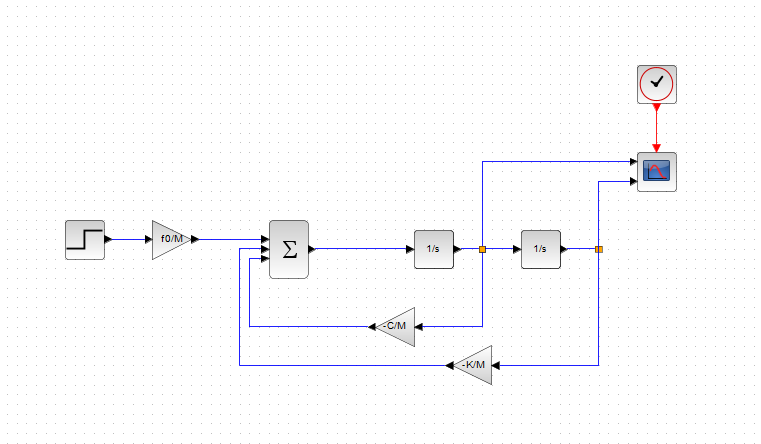
\includegraphics[width=10cm]{../graph/bane-model.png}
  \caption{作成したシミュレーションモデル}
  \label{fig:bane-model.png}
\end{figure}

このとき,左側の積分器の出力が$v(t)$であり,右側の積分器の出力が$x(t)$である.

\section{シミュレーション結果}
作成したシミュレーションモデルを用いて,図2のようなシミュレーション結果を得た.

使用した各定数は次のとおりである.
\begin{itemize}
  \item $m = 出席番号 \times 100$ = 420[kg]
  \item $k = \frac{|150 + (出席番号 - 25)^2 \times 50|}{10} = 1460$[kg/s$^2$]
  \item $c = 650 - (出席番号 - 25)^2 = 361$[kg/s]
  \item $f_o = 300$[kg $\cdot$ cm / s$^2$]
\end{itemize}

\begin{figure}[H]
  \centering
  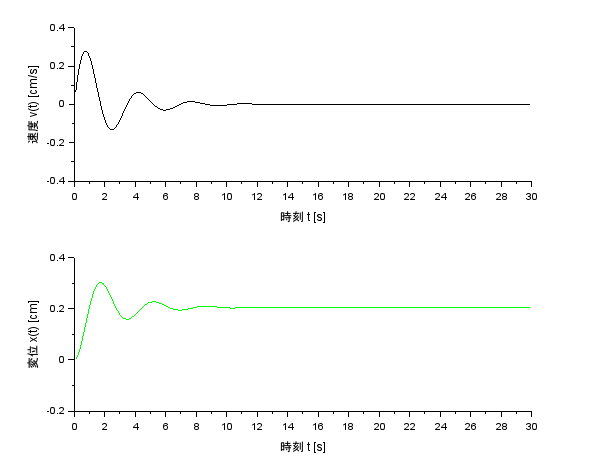
\includegraphics[width=10cm]{../graph/bane-graph.png}
  \caption{系の時間応答シミュレーション結果}
  \label{fig:bane-graph.png}
\end{figure}

\section{結果の評価}
まず,質量は正のステップ入力に対し,$x(t)$が正の方向に変位し,また,加速により$v(t)$が正となることは間違いない.
少なくともこの観点には,図2の出力は沿った結果となっている.

次に,定常応答について評価する.
定常応答は,$t \rightarrow \infty$となったときの$x(t)$及び$v(t)$である.
質量は最終的に静止するはずであるから,$v(t)$の定常応答は0となるはずである.
一方,$x(t)$の定常応答は,バネによる弾性力とダンパによる抵抗力のバランスによって決定される.
$x(t)$の定常応答$x_\infty$は,$x_\infty = \frac{f_o}{k}$とすると,
$v(t)$が0となればダンパの抵抗力は発生しなくなることを考えれば,$x_\infty = \frac{300}{1460} = 0.205$[cm]となる.
これら2つの定常応答に対して,図2の出力は沿った結果となっている.

最終的にシミュレーションモデルの結果が正しいか判断するには,これに加え収束までの時間と,周波数について検討する必要があると考えられる.
しかし,今回は時間が足りなかったため,これらの検討は行わなかった.
したがってダンパ成分に対する評価が不十分である.

\begin{thebibliography}{99}
  \bibitem{ataka} 佐藤 拓史、実験テキスト「数値シュミレーション」、(2022年),
\end{thebibliography}

\end{document}